\chapter{Separazione dei BTX}
La miscela dei BTX\footnote{Con \textit{BTX} viene intesa la miscela di aromatici a basso peso molecolare, quindi benzene, toluene, xileni e etilbenzene.} viene facilmente separata inizialmente tramite una rettifica in tre frazioni, rispettivamente composte da benzene ($T_{eb}=80^oC$ circa 60 piatti), toluene ($T_{eb}=110.6^oC$ circa 60 piatti) e xileni e etilbenzene ($T_{eb}=136.2 - 144.4^oC$).

\section{Separazione degli aromatici dagli altri idrocarburi}
Dato il basso range di temperature in cui si trovano tutte le specie che confluiscono nell'impianto di separazione (posizionato subito dopo l'impianto di reforming, che produce una elevata quantit� di aromatici), non � possibile operare con una semplice rettifica anche per l'elevato numero di azeotropi che si formano. si opera, quindi, sfruttando la maggiore polarizzabilit� dei composti aromatici rispetto ai composti paraffinici, si usa quindi un solvente che abbia le seguenti caratteristiche:
\begin{itemize}
	\item Sciolga facilmente e bene i composti aromatici
	\item Non sia completamente miscibile con la frazione idrocarburica
	\item Sia facilmente separabile dal prodotto (per esempio per distillazione)
\end{itemize}
come solventi sono stati scelti, per le loro caratteristiche quelli riportati in \tablename~\ref{tab:btx:solventiEstrazione}
\begin{table}[htbp]
	\centering
		\begin{tabular}{p{5cm}cc} \hline
			Sostanza									&		B.P.		&		Densit�	\\
																&	$T [^oC]$	&		$Kg/L$	\\ \hline
			Glicole dietilenico				& 245 			& 1.05 \\
			\hbox{\pentamethylene{3==O}{1W==OH;5W==OH}} & & \\
			Dimetilsolfossido 				& 190 			& 1.21 \\
			\hbox{\dimethylenei[a]{1==S;2==O}{1==$CH_3$;1W==$CH_3$}} & & \\
			Sulfolano  								& 286 			& 1.26 \\
			\hbox{\fiveheterovi{1==S}{1Sa==O;1Sb==O}} & & \\
			n-formilmorfolina	 				& 2.43 			& 1.15 \\ 
			\hbox{\sixheterovi{1==N;4==O}{1==CHO}} & & \\ \hline
		\end{tabular}
	\caption{Solventi utilizzati per la separazione dei BTX}
	\label{tab:btx:solventiEstrazione}
\end{table}
Uno schema semplificato e abbastanza generico � visibile in \figurename~\ref{fig:btx:extractionPlant}, dove si vede il posizionamento dell'impianto di estrazione degli aromatici all'interno di un impianto di raffineria. I differenti processi utilizzati si basano sull'uso di solventi differenti e le diverse tecniche di separazione dei prodotti.
\begin{figure}[htbp]
	\centering
		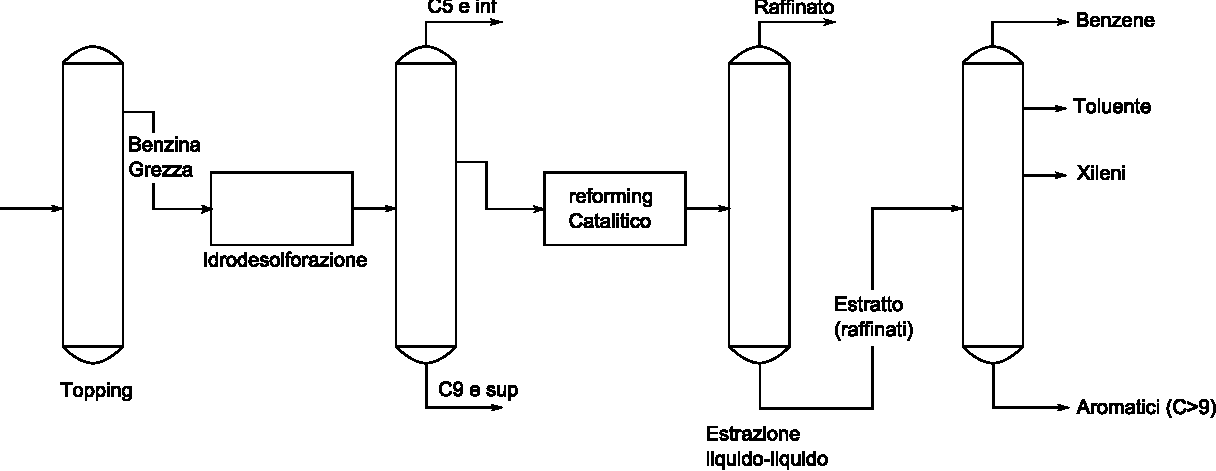
\includegraphics[width=0.80\textwidth]{image/ImpiantoEstrazioneBTX}
	\caption{Rappresentazione della posizione dell'impianto di estrazione di BTX in una raffineria}
	\label{fig:btx:extractionPlant}
\end{figure}

\subsection{Processo UDEX}
\'E il primo processo utilizzato per l'estrazione dei BTX dalla frazione idrocarburica; in questo caso il solvente e l'idrocarburo viaggiano in controcorrente, pertanto per migliorare la prestazioni nella parte finale della colonna viene effettuato un riflusso degli aromatici.

Come solvente viene utilizzato glicole dietilenico con l'aggiunta di acqua per migliorarne ulteriormente le caratteristiche di immiscibilit�; questa non potrebbe essere utilizzata da sola, sia a causa della temperatura di ebollizione che dalla bassa solubilit� con composti aromatici. La temperatura operativa � di circa $175^oC$, mentre la pressione � mantenuta a circa 8bar.

Lo schema dell'impianto � visibile in \figurename~\ref{fig:btx:UDEXPlant}, dove sono evidenti le apparecchiature principali e i flussi, l'alimentazione viene inviata, come gi� detto, in controcorrente con il solvente (DEG miscelato ad acqua), all'uscita dall'estrattore si hanno, come frazione leggera il raffinato composto dall'alimentazione a cui sono stati sottratti gli aromatici, mentre dalla coda esce il solvente contenete gli aromatici. Questo viene inviato allo stripper che opera alla stessa temperatura, ma a pressione inferiore effettuando quindi una distillazione flash. Dalla testa usciranno i composti aromatici e l'acqua mentre dalla coda il solvente che viene rinviato all'estrattore. La miscela acqua/aromatici viene fatta condensare (tramite abbassamento delle temperature) e successivamente inviata ad uno smiscelatore, da cui vengono allontanati i composti aromatici che in parte vengono inviati come riflusso all'estrattore, e in parte sottratti come prodotto. l'acqua uscente dal separatore viene riciclata.
\begin{figure}[htbp]
	\centering
		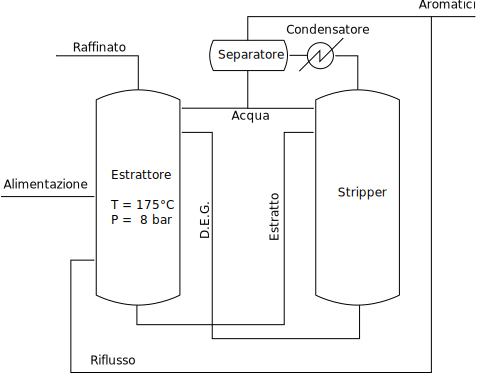
\includegraphics[width=0.60\textwidth]{image/ImpiantoUDEX}
	\caption{Rappresentazione dell'impianto UDEX}
	\label{fig:btx:UDEXPlant}
\end{figure}

Gli impianti sviluppati successivamente sono tutti perfezionamenti di questa tipologia di impianto.

\subsection{Processo SNAM-Progetti}
L'impianto realizzato dalla SNAM-Progetti ricalca lo schema dell'impianto BTX ma utilizza dimetilformalina come solvente e introduce altre due apparecchiature per il recupero del solvente presente nel raffinato e uno stripper iniziale per spingere la selettivit� rimandando all'estrattore le paraffine. Lo schema di processo � visibile in \figurename~\ref{fig:btx:SNAMPlant}, dove sono ben evidenti gli elementi principali dell'impianto.

La carica iniziale viene inviata ad un estrattore in cui il solvente (dimetilformalina) procede controcorrente, dalla testa esce la carica idrocarburica che viene mandata ad una seconda colonna di estrazione, in questo caso il solvente � costituito da acqua che asporta anche le ultime traccie di dimetilformalina dalla miscela idrocarburica.

Il solvente contenente gli aromatici viene dapprima inviato ad uno stripper che elimina le tracce di idrocarburi presenti e le reinvia all'estrattore primario, mentre il solvente contenete i BTX viene inviato ad una seconda colonna di stripping per la separazione dei BTX (e acqua) dal solvente; questo viene rinviato alla colonna di estrazione, mentre i BTX e l'acqua subiscono smiscelazione e separazione, ma mentre i BTX vengono eliminati dal processo (sono il prodotto desiderato), l'acqua prima di ritornare nell'estrattore confluisce (in parte) nella colonna di lavaggio del raffinato vista inizialmente per recuperare il solvente.
\begin{figure}[htbp]
	\centering
		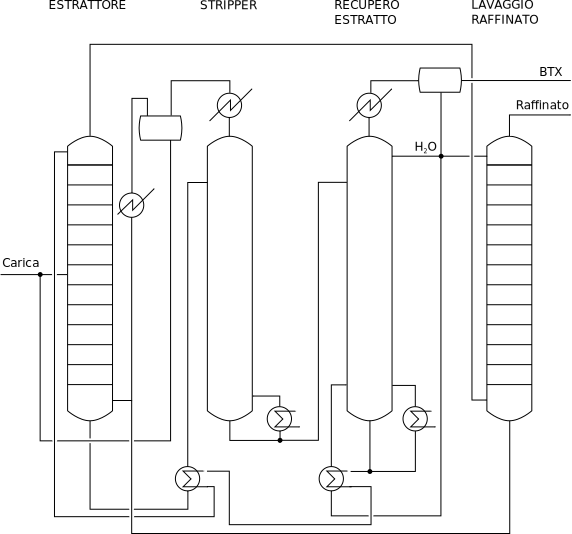
\includegraphics[width=0.80\textwidth]{image/ImpiantoBTX_SNAM}
	\caption{Rappresentazione dell'impianto SNAM}
	\label{fig:btx:SNAMPlant}
\end{figure}

\subsection{Processo IFP}
Il processo IFP\footnote{Istituto Francese Petroli} utilizza come solvente il dimetilsolfossido e l'estrazione viene compiuta in una colonna a piatti rotanti, dove � la forza centrifuga (gestibile dagli operatori) a far si che vi sia un flusso controcorrente.

Al posto dello stripping per il recupero del solvente si opera usando butano, che avendo densit� inferiore, far� si che il funzionamento sia a flussi invertiti (il solvente fuoriesce dall'alto della colonna). A seguito vi saranno una serie di colonne di lavaggio con acqua e di debutanazione per il recupero del flusso del'estrattore del dimetilsolfossido.

\subsection{Altri processi}
Il processo \textit{Lurgi} non passa attraverso una semplice estrazione dei BTX, ma si procede con una distillazione estrattiva, il cui solvente � composto da NMP\footnote{N-metilpirrolidone = \sixheterovi{3==N}{3==CH$_3$}}.
Anche in questo caso a seguito della distillazione estrattiva (dalla cui testa escono i composti non aromatici) si ha separazione dei BTX dal solvente tramite una rettifica.

Un'ulteriore tecnica utilizzata � la distillazione azeotropica in cui il solvente � costituito da metanolo che da luogo ad una miscela azeotropica con i composti non aromatici, si ha quindi una separazione di questi dagli aromatici. Il metanolo viene recuperato con acqua e successivamente separato (con notevoli costi energetici per l'intero processo). Questo procedimento viene adottato qualora la concentrazione del toluene sia superiore al 40\%.

\section{Separazione degli xileni}
Una volta ottenuta la miscela di BTX dalla prima separazione si pu� procedere alla distillazione per ottenere benzene, toluene e la miscela di xileni contenente anche etilbenzene e stirene. Da quest'ultima, per gli scopi dell'industria chimica, � necessario procede ad una ulteriore separazione dei componenti della miscela degli xileni e dell'etilbenzene, in particolare � necessario ottenere i tre differenti xileni\footnote{ovvero \textit{orto}, \textit{meta} e \textit{para} xilene}, l'etilbenzene e lo stirene puri. Data la vicinanza delle temperature di ebollizione e cristallizzazione delle diverse specie (\tablename~\ref{tab:btx:temperatureEbCr}) la separazione � assai difficoltosa, infatti per separare \ce{\textit{p}-xilene} e \ce{\textit{m}-xilene} servirebbe una colonna di circa 800 piatti. Non � nemmeno possibile procedere facilmente per estrazione data la somiglianza dei composti considerati (polarit� praticamente identiche), ma comunque possibile operare un adsorbimento frazionato.
\begin{table}[htbp]
	\centering
		\begin{tabular}{lcc} \hline
										& Ebollizione			& Fusione					\\ 
			Componente		&	$T_{eb}$, $^o$C	&	$T_{f}$, $^o$C	\\ \hline
			Etilbenzene		&	136.2						& -95.0						\\
			\textit{p}-xilene			& 138.3						& ~13.3						\\
			\textit{m}-xilene			& 139.1						& -47.9						\\
			\textit{o}-xilene			& 144.4						& -25.2						\\
			Stirene				& 145.2						& 								\\ \hline
		\end{tabular}
	\caption{Temperature di ebollizione e cristallizzazioen dei BTX}
	\label{tab:btx:temperatureEbCr}
\end{table}

\subsection{Cristalliazzazione frazionata }
Come � evidente da \figurename~\ref{fig:btx:cristallizzazione} la miscela si \textit{p}-xilene e \textit{m}-xilene pu� essere separata tramite cristallizzazione, ma si ha la formazione di un eutettico all'86\% composto da \textit{m}-xilene e di conseguenza una sola cristallizzazione non permette di ottenere una purezza del prodotto sufficiente. Per ovviare a ci� si pu� procedere ricristallizzando il prodotto iniziale o effettuando un lavaggio dei cristalli per eliminare il liquido intersitizale.
\begin{figure}[htbp]
	\centering
		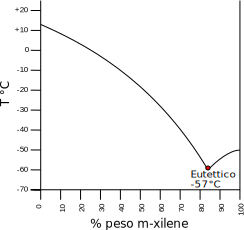
\includegraphics[width=0.60\textwidth]{image/eutettico}
	\caption{Temperatura di fusione del sistema \textit{p}-xilene \textit{m}-xilene}
	\label{fig:btx:cristallizzazione}
\end{figure}

La separazione mediante cristallizzazione viene realizzata in un impianto secondo un processo chiamato \textit{Phillips} in cui la separazione del liquido interstiziale dai cristalli di \textit{p}-xilene viene realizzato tramite ricristallizzazione e ulteriore rettifica, o in un impianto \textit{Atlantic} in cui si utilizza un solvente per eliminare dai cristalli di \textit{p}-xilene il liquido interstiziale (separati poi tramite rettifica).

\subsubsection{Impianto Phillips}
In questa tipologia di impianto (rappresentato in \figurename~\ref{fig:btx:phillipsPlant}) la miscela iniziale contenente i componenti aromatici $C_8$ viene inviata ad una prima colonna di distillazione (\textit{A}) composta da circa 150 piatti dalla cui coda si ottiene l'\textit{o}-xilene con una purezza sufficientemente elevata (circa il 98\%).

La testa della coda viene inviata ad una colonna di rettifica composta da circa 350 piatti (\textit{B}), chiamato anche \textit{superfrazionatore}\footnote{A volte si preferisce sostituire a questo un impianto per l'isomerizzazione da etilene a xileni.}, dalla cui testa si ottiene etilbenzene mentre dalla coda si ricava la miscela di meta e para xilene. Questa viene dapprima raffreddata fino ad una temperatura di circa $-23^oC$ (sfruttando il riscaldamento della miscela gi� raffreddata di recupero) e successivamente tramite un ciclo ad etilene fino a $-54^oC$.

La miscela cos� raffreddata viene inviata ad un filtro rotante dove si separano i cristalli di \textit{p}-xilene mentre la fase liquida � composta da \textit{m}-xilene che viene dapprima sottoposta ad una rettifica in una colonna da 200 piatti (\textit{C}) per recuperare altro etilbenzene dalla testa, mentre la coda viene inviata ad una altra colonna di rettifica di circa 50 piatti (\textit{D}) dalla cui testa si ricava \textit{m}-xilene al 95\%.

I cristalli di \textit{p}-xilene dopo una prima fusione vengono ricristallizzati e l'effluente inviato ad una colonna di rettifica (\textit{E}) dalla cui coda si ricava \textit{p}-xilene al 98\% e dalla cui testa si recupera una miscela di meta e para xileni che viene reciclata.

La colonna di purificazione \textit{E} pu� anche essere sostituita da una colonna a pistone con fondo riscaldato, in pratica un pistone preme sul fondo i cristalli in modo che i cristalli impuri si fondano alla base creando due gradienti, un primo di temperatura dal fondo verso la testa della colonna e del \textit{p}-xilene che tende verso il fondo della colonna (mentre il \textit{m}-xilene tende verso la testa).
\begin{figure}[htbp]
	\centering
		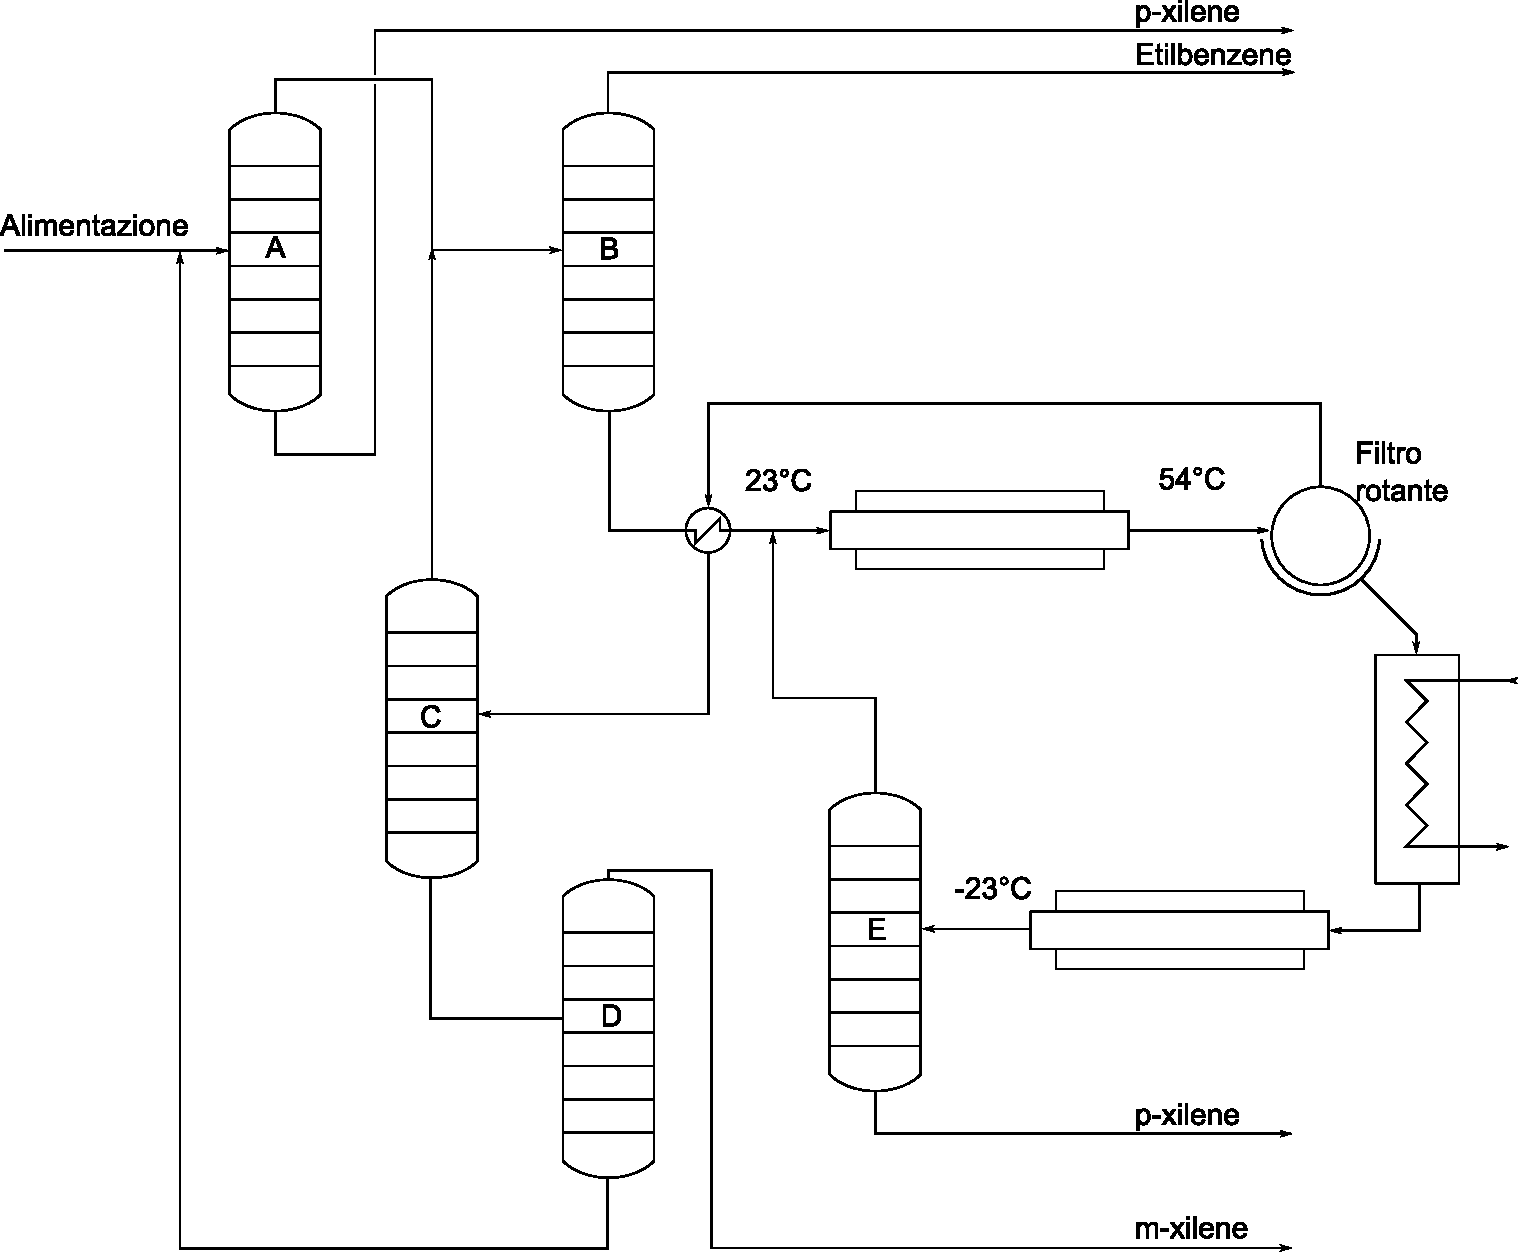
\includegraphics[width=0.90\textwidth]{image/phillipsPlant}
	\caption{Impianto per la separazione \textit{p}-xilene \textit{m}-xilene secondo il processo Phillips}
	\label{fig:btx:phillipsPlant}
\end{figure}

\subsubsection{Impianto Atlantic-Richfield}
In questa tipologia di impianto si procede alla separazione del \textit{p}-xilene dal \textit{m}-xilene non tramite ricristallizzazione e successiva rettifica, ma per mezzo di un lavaggio dei cristalli con toluene. Questo viene poi separato dal toluene tramite una rettifica.

\subsection{Adsorbimento frazionato}
In questo processo viene sfruttata la capacit� dei composti di adsorbire alcune sostanze, in questo caso particolare vengono usati dei setacci molecolari costituiti da \textit{silico-alluminati} con una microgeometria molto controllata.

Il \textit{p}-xilene riesce a penetrare nei setacci zeolitici, mentre il \textit{m}-xilene a causa degli ingombri sterici, non riesce a penetrare negli interstizi. Al termine di questo adsorbimento vengono separate le fasi liquide e solide (che hanno intrappolato il \textit{m}-xilene). Dai setacci si ha eliminazione del \textit{p}-xilene usando toluene come eluente, si ottiene cos� una soluzione di \textit{p}-xilene e toluene che poi verr� separata mediante rettifica. I setacci molecolari vengono poi rinviati alla fase di adsorbimento.

Questo schema ideale (\figurename~\ref{fig:btx:adsorbimentoFrazionatoIdeale}) sarebbe realizzabile se la fase contenente i setacci molecolari fossero liquida; il fatto che si tratti di una fase solida comporta una serie di problematiche che sono state risolte ricorrendo ad una configurazione chiamata SMB\footnote{Simulated Moving Bed}. In questo caso la colonna di adsorbimento/desorbimento � suddivisa in una serie di piatti e riempita da granuli di silico-alluminati. Ogni piatto conterr� un ingresso e una uscita e tutte queste sono collegate ad una valvola rotante.

La valvola rotante si occupa di modificare ciclicamente i flussi in ingresso e uscita da ogni piatto (alternativamente in ingresso si avr� la miscela di \textit{m}-xilene e \textit{p}-xilene oppure toluene e in uscita si avr� il raffinato o l'estratto), creando cos� un processo quasi continuo (idealmente continuo se il numero di piatti tende ad $\infty$).

Il raffinato, composto da \textit{m}-xilene non viene utilizzato tal quale ma subisce una isomerizzazione, reazione praticamente atermica, con catalizzatori acidi (zeolitici) e il prodotto verr� riciclato per ottenere il solo \textit{p}-xilene. La possibilit� di cracking dato dal catalizzatore utilizzato viene minimizzato aggiungendo idrogeno, che viene poi recuperato.

\begin{figure}[htbp]
	\centering
		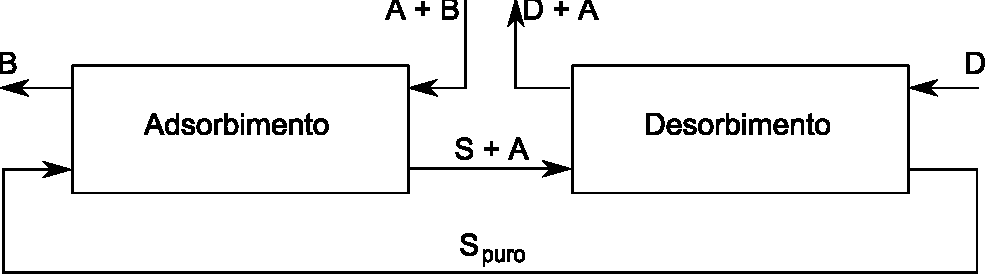
\includegraphics[width=0.90\textwidth]{image/adsorbimentoFrazionatoIdeale}
	\caption[Schema di un impianto di asorbimento frazionato ideale]{Schema di un impianto di asorbimento frazionato ideale. \textit{A}:~\textit{p}-xilene; \textit{B}:~\textit{m}-xilene; \textit{D}:~toluene; \textit{S}:~silico-alluminati}
	\label{fig:btx:adsorbimentoFrazionatoIdeale}
\end{figure}

\begin{figure}[htbp]
	\centering
		
\includegraphics[width=0.90\textwidth]{image/adsorbimentoFrazionato}
	\caption[Schema di un impianto di asorbimento frazionato. Processo Parex]{Schema di un impianto di asorbimento frazionato secondo il processo \textit{Parex}. \textit{A}:~\textit{p}-xilene; \textit{B}:~\textit{m}-xilene; \textit{D}:~toluene;}
	\label{fig:btx:adsorbimentoFrazionato}
\end{figure}